\documentclass[12pt]{article}

\usepackage{graphicx}
\usepackage{float}
\usepackage{amsmath}
\usepackage{amssymb}
\usepackage{graphicx}
\usepackage[utf8]{inputenc}
\usepackage[spanish]{babel}
\usepackage{geometry}
\geometry{left=2cm,right=2cm,top=2cm,bottom=2cm}
\usepackage{listings}
\lstset{basicstyle=\ttfamily,
  showstringspaces=false,
  commentstyle=\color{red},
  keywordstyle=\color{blue}
}


\title{%
  Luz y sombreado\\
  \large Tarea 04 \\
    \Large Computación Gráfica\\
     \large UNAM 2022-2}
\author{Gibran Zazueta Cruz \\
\small 15/marzo/2022}
\date{}

\begin{document}
\maketitle

\section{Introducción}


\subsection{Modelo de luz}

El modelo de luz utilizado se compone de una componente ambiental, una difusa y una especular.

\begin{figure}[H]
\centering
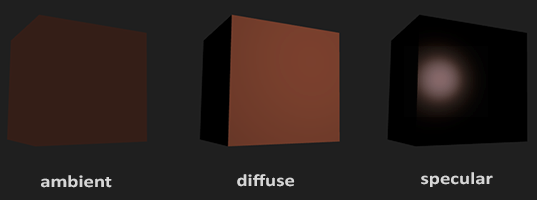
\includegraphics[scale=0.5]{images/lighting.png}
\caption{Componenetes de luz \cite{open}}
\end{figure}



Para la imlementacion se utilizaron los siguientes parametros

\subsubsection{Ambiental}

La luz ambiental es una luz que ilumina de manera homogénea todos los objetos de la escena.

Se calcula como

\begin{equation}
I_{A}=\kappa_{A}\Lambda_{A}
\end{equation}

En la implementación se utilizó $I_{A}=100$ y $\kappa_{A}=[0.3,0.3,0.3]$

\subsubsection{Difusa}

La iluminación difusa le da mayor iluminación a las zonas del objeto alineadas hacia la fuente de luz. Ee decir la luz muestra una especie de \textit{dirección} sobre el objeto.

La luz difusa se calcula como 

\begin{equation}
I_{D}=\kappa_{D}\Lambda_{D}(\vec{n} \cdot \vec{l})
\end{equation}

donde $\vec{n}$ es la normal del vértice de incidencia y $\vec{l}$ es el vector de dirección de la fuente de luz sobre el vértice.

En la implementación se utilizaron 2 fuentes de luz difusa. Una con luz blanca e intensidad $\Lambda_{D_{1}}=10$. La otra ocn luz roja e intensidad $\Lambda_{D_{2}}=80$. Ambas están localizada en la posición $[10,10,10]$

El coeficiente $\kappa$ del objeto se consideró como $\kappa_{D}=[0.07568, 0.61424,0.07568]$

\subsubsection{Especular}

La luz especular está basada en la propiedad reflectiva de la luz al incidir sobre un objeto. Para la visualización de su efecto se deberá definir un observador dentro de la escena.

El calcula es el siguiente

\begin{equation} \label{eq:3}
I_{E}=\kappa_{E}\Lambda_{E}(\vec{o} \cdot \vec{l})^{\rho}
\end{equation}

donde $\vec{o}$ es el vector de dirección del observador. La ecuación (3) también se puede escribir

\begin{equation}
I_{E}=\kappa_{E}\Lambda_{E}(\vec{o} \cdot \vec{h})^{\rho}
\end{equation}


donde $h=2(\vec{o} \cdot \vec{l})\vec{n}-\vec{l}$

Para la implementación se utilizó una luz especular blanca con intensidad 2 y en la posición [10,10,10]
 
El coefieciente del objeto para luz especular fue: $ke={0.633, 0.72811,0.66};$

\subsection{Gouraud Shading}

EL sombreado de Gouraud es un método para sombrear la superficie de un polígono, de acuerdo a un modelo de luz implementado.

Los pasos son:

\begin{itemize}
\item Calcular los vectores normales en los vértices del polígono
\item Calcular la iluminación en cada vértice
\item Interpolar el valor de iluminación entre vértices (formar border
\item Interpolar la iluminación entre los bordes para rellenar el pológono (scan conversion)
\end{itemize}



\subsection{Phong Shading}


Phong en un método de sombreado más sofisticado que Gouraud.

La diferencia principal es que la interpolación entre vértices es del valor de sus normales

Los pasos para el sombredo de phong son:

\begin{itemize}
\item Calcular los vectores normales en los vértices del polígono
\item Interpolar las normales sobre la superficie del polígono
\item Calcular la iluminación en cada normal (punto) de la superficie.

\end{itemize}
 
 
 Para esta implementación también se realizó interpolación lineal del vector $\vec{l}$ y $\vec{o}$

\section{Estructura del código}

El programa tiene como base el código de la tarea 3.\\

En lights.h se define la clase \textit{lights} para representar las luces de la escena. Cada objeto tiene intensidad, posición y color.

En \textit{mainwindow.cpp} se crean los objetos de luz para luz blanca, luz roja y luz especular

En la clase \textit{cubeobject} se calculan las normales de las caras del cubo. Dspués las normales de cada vertice, haciendo un promedio de las normlaes de sus caras colindantes.

En \textit{CamProjection.cpp} la función \textit{projectPoint} recibe como entrada el objeto (cuboide) y las luces de la escena. Además de proyectar los punto y realizar scan conversion, aqui se calcula la intensidad de la luz y el ocmbreado de la superficie.

Para gouraud se calcula el color en los 8 vértices del cuboide. Para ello se utiliza la función calcLightVertex de \textit{shading.h} que implementa las ecuaciones $(1), (2)$ y $(3)$. 
Después se interpolan los valores de intensidad de los vértices en el mismo método de scan conversion

Para Phong, se calculan las normales $\vec{n}$ de los vértices, el vector $\vec{l}$ entre cada vértice con la posición de la luz y el vector $\vec{o}$ entre cada vértice con la posición del observador. Se interpolan estos valores sobre la superficie dentro del método de scan conversion

\section{Ejecutar el programa}
En la carpeta de build se puede ejecutar el programa con el archivo lightingShading-Run. Desde la consola de comandos de linux:

\begin{lstlisting}[language=bash,title={bash}]
./lightingShading-Run
\end{lstlisting}


En la carpeta principal está el código fuente. Para generar el ejecutable primero se genera el Makefile con

\begin{lstlisting}[language=bash,title={bash}]
 qmake lightingShading.pro
\end{lstlisting}

Después se construye el proyecto con \textit{make}



\section{Instrucciones de uso}
Se presenta la interfaz del programa.

\begin{figure}[H]
\centering
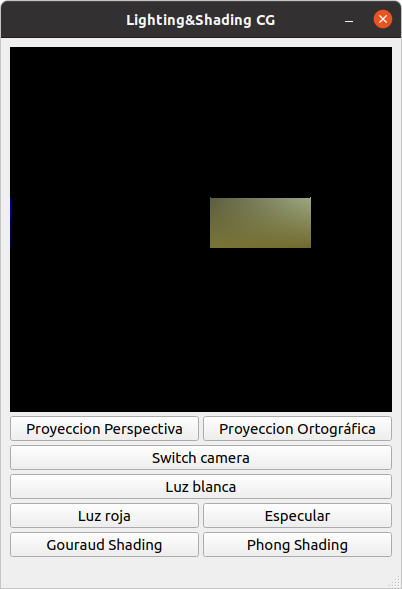
\includegraphics[scale=0.5]{images/gui.png}
\caption{Interfaz gráfica del programa}
\end{figure}

Al presionar \textit{Proyeccion Perspectiva} o \textit{Proyeccion Ortografica} se cambia al tipo de proyección correspondiente.

\textit{SWitch camera} cambia el renderizado entre la cámara 1 y la cámara 2

Los botones \textit{Luz blanca}, \textit{Luz Roja} y \textit{Especular} encienden o apagan las luces correspondientes. El programa inicia con todas las luces activas.

Finalmente \textit{Gouraud Shading} activa el combreado por Gouraud y \textit{Phong Shading} el sombreado de Phong.



\section{Programa en ejecución}

\begin{figure}[H]
\centering
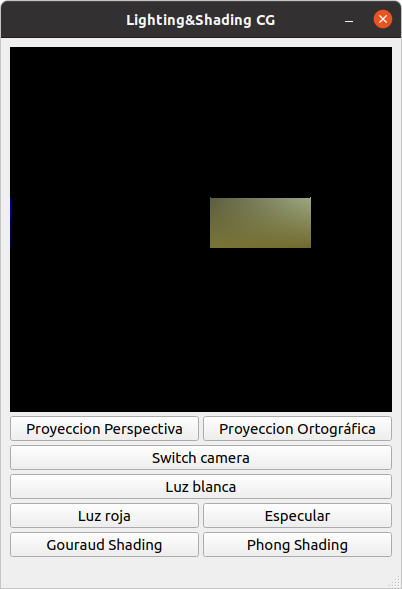
\includegraphics[scale=0.5]{images/ej1.png}
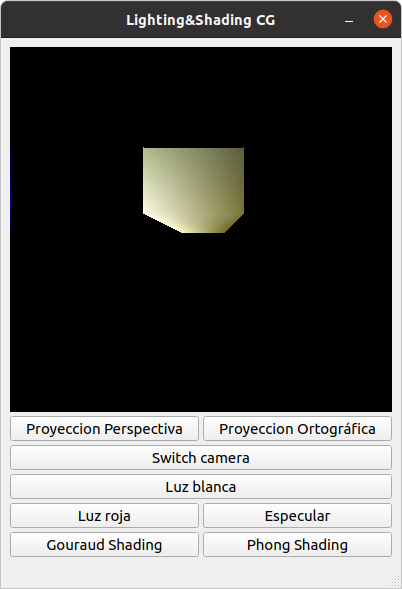
\includegraphics[scale=0.5]{images/ej2.png}
\caption{Gouraud Shading. Cámara 1 y 2. Proyectado en perspectiva}
\end{figure}


\begin{figure}[H]
\centering
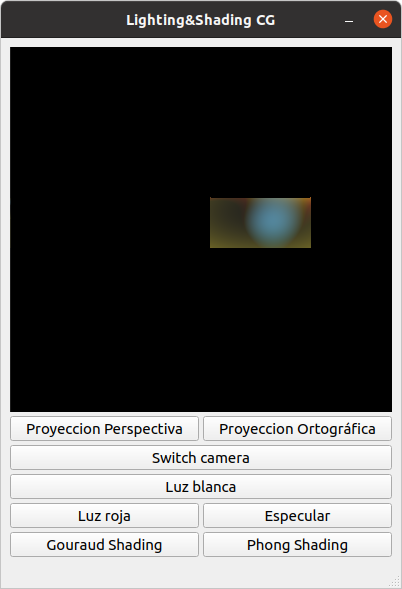
\includegraphics[scale=0.5]{images/ej3.png}
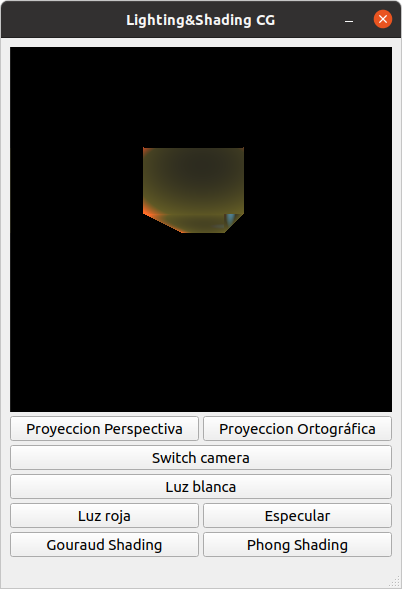
\includegraphics[scale=0.5]{images/ej4.png}
\caption{Phong Shading. Cámara 1 y 2. Proyectado en perspectiva}
\end{figure}



\begin{figure}[H]
\centering
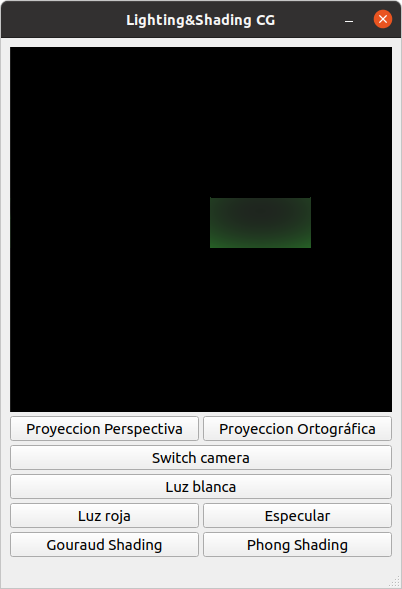
\includegraphics[scale=0.5]{images/ej5.png}
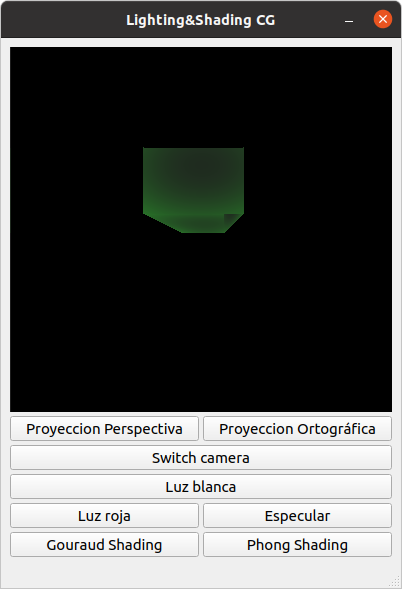
\includegraphics[scale=0.5]{images/ej6.png}
\caption{Phong Shading. Solo luz blanca. Cámara 1 y 2. Proyectado en perspectiva}
\end{figure}


\begin{thebibliography}{99}


\bibitem{open} Learn OpenGL. Basic Lighting ($https://learnopengl.com/Lighting/Basic-Lighting$)

\end{thebibliography}


\end{document}